% !TEX root = ../SCXMLREF.tex


\section{Intrusion Detection System}
\label{sec:secbot}

An \IDS is used to illustrate the use of refinement in \statecharts and how it is supported by \EventB verification tools.
The \IDS is designed using an \ASIC which connects to a buzzer and a sensor over a \SPI bus. The system is controlled via the \ASIC on the \SPI bus. At power-up, the \ASIC sends commands over the \SPI bus to initialise the sensor and the buzzer. After waiting for 50 milliseconds the \ASIC enters its main routine, which makes the buzzer respond to the sensor. In the early design phase the \statechart model of this system may be limited to the \ASIC that captures the initialisation of the peripherals and the 50 ms wait. In the interest of simplicity, we elide all details of the main routine.

A \statechart model of this system is shown in Fig.~\ref{fig:ASIC}. The \ASIC starts by initialising the buzzer; this involves sending a message over the \SPI bus. These messages constitute an implementation detail that we elide at this abstraction level. Once the message is sent (which will be indicated by some event saying that the \SPI system is done), the \ASIC moves on to initialise the sensor. After that the \ASIC moves into a waiting state for 50 ms, and finally moves into the state which represents normal operation. \KarlaAdd{At this abstraction the} \textbf{spi\_done} \KarlaAdd{trigger, which indicates that the }\SPI \KarlaAdd{system has finished, is an internal trigger that can be fired at any time.} \KarlaDelete{At this abstraction the spi done triggered, which signals completion by the SPI system, is an internal trigger that can be fired at any time.}

In a subsequent level of refinement, shown in Fig.~\ref{fig:ASIC_SPI_1}, the designer \KarlaAdd{uses superposition refinement to} add\KarlaDelete{s} a parallel state representing the \SPI subsystem. The \SPI subsystem is usually \SonChange{on}{in} an \textbf{Idle} state until the \textbf{send\_message} trigger is raised, at which point the \SPI subsystem enters a state \textbf{Sending Message}, which represents sending the message, byte by byte. When the last byte of the message is sent, it raises the \textbf{spi\_done} trigger, allowing the other parallel state to continue, while \SonAdd{the} \SPI subsystem returns to idle. In the current refined model we have incorporated the implementation details for raising \textbf{spi\_done} and introduced a new internal trigger 
\textbf{send\_message}, which is nondeterministic at this point.

\begin{figure*}[!tb]\centering
	    \begin{subfigure}[t]{0.3\textwidth}
	        \begin{centering}
	        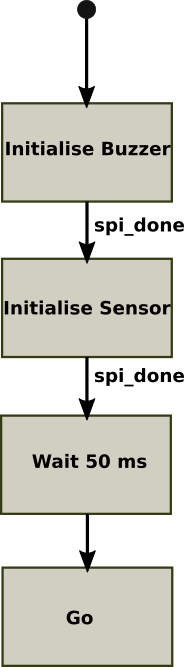
\includegraphics[height=2.5in]{figures/ASIC}
	        \caption{\ASIC component high level abstraction}
	        \label{fig:ASIC}
	        \end{centering}
	    \end{subfigure}
\qquad
	    \begin{subfigure}[t]{0.5\textwidth}
	        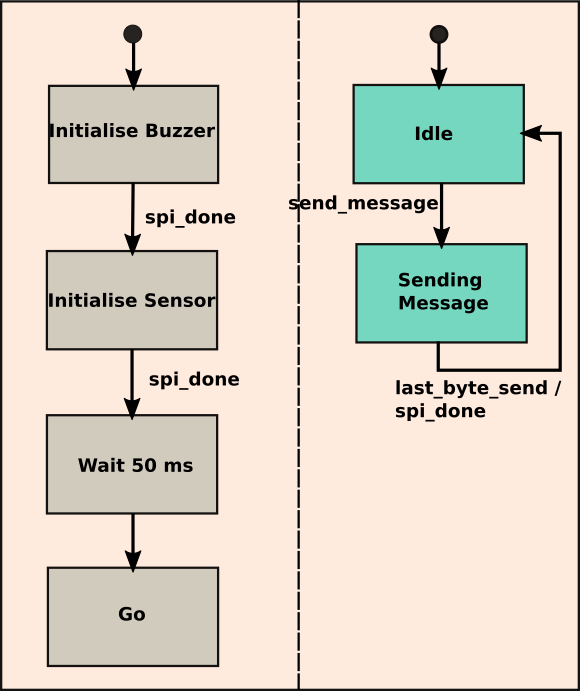
\includegraphics[height=2.5in]{figures/ASIC&SPI_1}
	        \caption{First refinement introducing the abstract model of the \SPI subsystem.}
	        \label{fig:ASIC_SPI_1}
	    \end{subfigure}
	    \caption{\Statechart diagram for \IDS including the abstract representation of the \ASIC and \SPI components.}
\end{figure*}

The model can be further refined by incorporating more details on how the initialisation states, the wait state, and the \SPI subsystem operate, including how they interact with each other. The \statechart diagram for this refinement level is in Fig.~\ref{fig:ASIC_SPI_2}. The \textbf{Initialise Buzzer} state constructs the \SPI message to send, then raises the \textbf{send\_message} trigger, and then waits.
After \textbf{send\_message} is raised, the \SPI subsystem reacts. It spins for a while in the \textbf{Send Byte} state, looping as many times as it takes to get to the last byte in the message. When the last byte in the message is sent, it goes back to \textbf{Idle} and raises an event which allows the state machine on the left to proceed. The sensor is then initialised in a very similar manner to the buzzer. After both peripherals are initialised, the state machine goes into the \textbf{Wait 50 ms} state, where it increments a counter until it reaches some maximum, then exits.

\begin{figure}[!tbp]
  \begin{centering}
  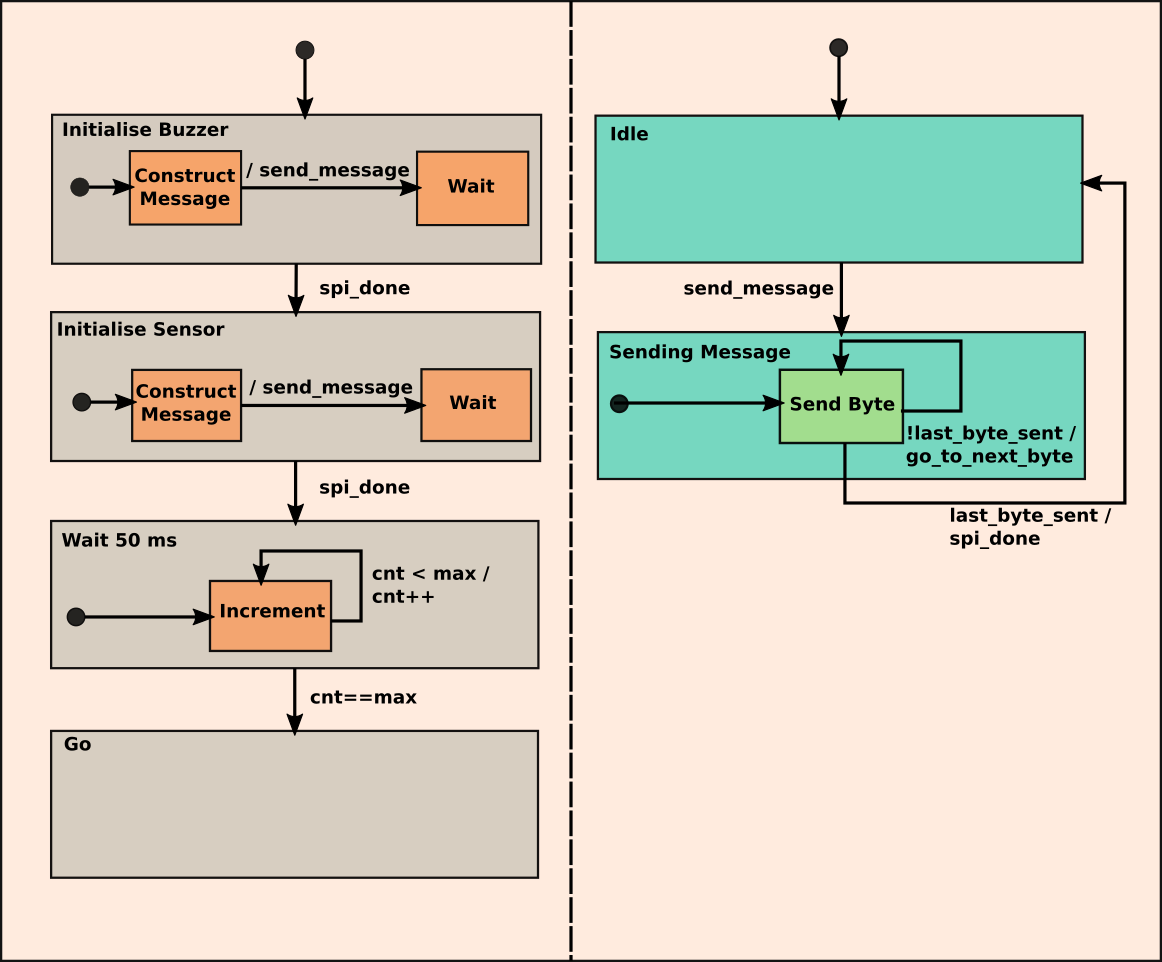
\includegraphics[width=0.8\textwidth]{figures/ASIC&SPI_2}
  \caption{\Statechart diagram for \IDS including implementation details for the messages sent between the system components.}
  \label{fig:ASIC_SPI_2}
  \end{centering}
\end{figure} 

The system described must send messages to complete the initialisation of the buzzer and sensor, but once the main routine is reached (\textbf{Go} state) no more messages should be sent through the \SPI bus. As a result, a desirable safety property is that \emph{when the \ASIC is in the \textbf{Go} state the \SPI subsystem
must be in the \textbf{Idle} state}.
\ColinChange{This safety property is introduced in the first refinement and maintained by subsequent refinements.}
{This safety property should hold from the first refinement and be preserved in all future refinements.}



%%% Local Variables:
%%% mode: latex
%%% TeX-master: "../SCXMLREF"
%%% End:

